\RequirePackage{luatex85}
\documentclass[preview]{standalone}
\usepackage{amsmath}
\usepackage{amssymb}
\usepackage[compat=1.1.0]{tikz-feynman}
%\usepackage{geometry,contour}
%\geometry{legalpaper, landscape, margin=0.05in}
%\paperheight 2.2in
%\paperwidth 4.5in



\begin{document}
\begin{center}
\begin{eqnarray}
\nonumber
\frac{df_Q}{dt} &=& \mathcal{C}^{2\leftrightarrow 2}_{>}[f_Q] {\color{red} +  \partial_p\left(A_Q p + \partial_p B_{Q}\right)_{<}f_Q}
\end{eqnarray}
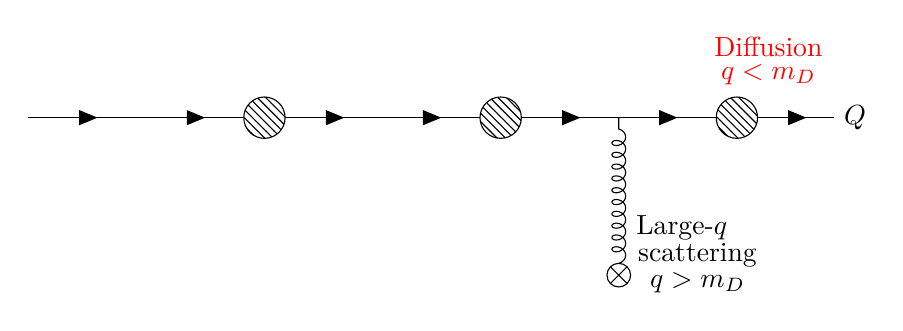
\begin{tikzpicture}
    \begin{feynman}
      \vertex (Qb) at (-7.5, -2);
      \vertex (Qc) at (-6, -2);
      \vertex[blob,scale=0.7] (Qcc) at (-4.5, -2) {};
      \vertex (Qd) at (-3, -2);
      \vertex[blob,scale=0.7] (Qdd) at (-1.5, -2) {};
      \vertex (Qe) at ( 0, -2);
      \vertex[blob,scale=0.7] (Qf) at ( 1.5, -2) {};
      \vertex (Qg) at ( 3, -2) {$Q$};
      \vertex[] () at (1.9, -1.1) {\color{red}Diffusion};
      \vertex[] () at (1.9, -1.45) {\color{red}$q<m_D$};
      \vertex[] () at (0.8, -3.4) {Large-$q$};
      \vertex[] () at (1., -3.75) {scattering};
      \vertex[] () at (1., -4.1) {$q>m_D$};
	  \vertex[crossed dot] (S1) at (0,-4) {};
      \diagram* {
       (Qb) -- [fermion] (Qc) -- [fermion] (Qcc) -- [fermion] (Qd) -- [fermion] (Qdd) -- [fermion] (Qe) -- [fermion] (Qf) -- [fermion] (Qg),
        (S1) -- [gluon] (Qe)
      };
    \end{feynman}
\end{tikzpicture}
\end{center}
\end{document}






